\documentclass[12pt]{article}


\usepackage{amssymb}
\usepackage{amsmath}
\usepackage{fullpage}
\usepackage{epsfig}
\usepackage{epstopdf, xcolor, hyperref}
\everymath{\displaystyle}
\usepackage{enumerate}

\newif\ifans

\anstrue

\begin{document}

\begin{center}
\underline{\LARGE{Relative and Absolute Extrema}}
\end{center}

\noindent SUGGESTED REFERENCE MATERIAL:

\bigskip

\noindent As you work through the problems listed below, you should reference Chapter 13.8 of the recommended textbook (or the equivalent chapter in your alternative textbook/online resource) and your lecture notes.

\bigskip

\noindent EXPECTED SKILLS:

\begin{itemize}

\item Be able to use partial derivatives to find critical points (possible locations of maxima or minima). 

\item Know how to use the Second Partials Test for functions of two variables to determine whether a critical point is a relative
maximum, relative minimum, or a saddle point. 

\item Be able to solve word problems involving maxima and minima. 

\item Know how to compute absolute maxima and minima on closed regions.

\end{itemize}

\noindent PRACTICE PROBLEMS:

\medskip

\noindent {\bf For problems 1-10, identify all critical points of the given function.  Then, classify each as the location of a  relative maximum, relative minimum, or saddle point.}

\begin{enumerate}

\item $g(x,y)=x^2+y^2-3x-4y+6$ 

\ifans{\fbox{Relative minimum at $\left(\frac{3}{2},2\right)$ }} \fi

\item $f(x,y)=x^2+4y^2-4y-2$ 

\ifans{\fbox{Relative minimum at $\left(0,\frac{1}{2}\right)$}} \fi

\item $g(x,y)=4x^2-3y^2+8x-9y-4$ 

\ifans{\fbox{Saddle point at $\left(-1,-\frac{3}{2}\right)$}} \fi

\item $f(x,y)=x^3-3x+y^2-6y$

\ifans{\fbox{Relative minimum at $(1,3)$; Saddle point at $(-1,3)$}} \fi

\item $h(x,y)=x^2-5xy+y^2$ 

\ifans{\fbox{Saddle point at $(0,0)$}} \fi

\item $f(x,y)=3x+y^2-e^x$

\ifans{\fbox{Saddle point at $(\ln{3},0)$}} \fi

\item $f(x,y)=x^6+y^6$

\ifans{\fbox{Relative minimum at $(0,0)$}} \fi

\item $f(x,y)=x^2y-6y^2-3x^2$

\ifans{\fbox{Relative maximum at $(0,0)$; Saddle points at $(6,3)$ and $(-6,3)$; Detailed Solution: \textcolor{blue}{\href{http://www.math.drexel.edu/classes/Calculus/resources/Math200HW/Solutions/15_200_Extrema_08.pdf}{Here}}}} \fi

\item $f(x,y)=x^3-3xy+\frac{1}{2}y^2$

\ifans{\fbox{Relative minimum at $(3,9)$; Saddle point at $(0,0)$}} \fi

\item $f(x,y)=\frac{1}{3}x^3-2x+x^2+2xy+y^2$

\ifans{\fbox{Relative minimum at $\left(\sqrt{2},-\sqrt{2}\right)$; Saddle point at $\left(-\sqrt{2},\sqrt{2}\right)$}} \fi

\item Consider $h(x,y)=3\sqrt{x^2+y^2}+6$

\begin{enumerate}

\item Explain why the Second Partials Test may not be used to locate the relative extrema/saddle points of $h(x,y)$.  

\ifans{\fbox{\parbox{1\linewidth}{$(0,0)$ is the only critical point of $h(x,y)$; but, the Second Partials Test does not apply because $h(x,y)$ does not have continuous second partial derivatives in any disk centered at this critical point.}}} \fi

\item Locate all relative maxima, relative minima, and saddle points, if any.

\ifans{\fbox{Relative minimum at $(0,0)$}} \fi

\end{enumerate}

\end{enumerate}

\noindent {\bf For problems 12-15, find the absolute extrema of the given function on the specified region $R$.}

\begin{enumerate}
\setcounter{enumi}{11}

\item $f(x,y)=5-4y-2x$; $R$ is the closed triangular region in the $xy$-plane with vertices $(3,0)$, $(0,1)$, and $(1,2)$. 

\ifans{\fbox{Absolute minimum of $-5$ at $(1,2)$; Absolute maximum of $1$ at $(0,1)$}} \fi

\item $f(x,y)=x^2-4xy+5y^2-8y$; $R$ is the closed triangular region with vertices $(0,0)$, $(3,0)$, and $(3,3)$.

\ifans{\fbox{Absolute minimum of $-11$ at $(3,2)$; Absolute maximum of 9 at $(3,0)$}} \fi

\item $g(x,y)=x^2-y^2-2x$; $R$: is the closed region in the $xy$-plane bounded by the graphs $y=x^2$ and $y=4$. 

\ifans{\fbox{\parbox{0.9\linewidth}{Absolute minimum of $-17$ at $(1,4)$; Absolute maximum of $2$ at $(-1,1)$; 
\\Detailed Solution: \textcolor{blue}{\href{http://www.math.drexel.edu/classes/Calculus/resources/Math200HW/Solutions/15_200_Extrema_14.pdf}{Here}}}} }\fi

\item $f(x,y)=x^2+xy+y^2$; $R$ is the closed square region defined by $-1 \leq x \leq 1$, $-1 \leq y \leq 1$.

\ifans{\fbox{Absolute minimum of 0 at $(0,0)$; Absolute maximum of 3 at $(1,1)$ and $(-1,-1)$}} \fi

\item A closed rectangular box with a volume of 16 $\text{ft}^3$ is made from two kinds of materials.  The top and bottom are made of material costing \$0.10 per square foot and the sides are made of material costing \$0.05 per square foot.  Find the dimensions of the box so the cost is minimized.

\ifans{\fbox{$2\text{ft} \times 2\text{ft} \times 4\text{ft}$; Detailed Solution: \textcolor{blue}{\href{http://www.math.drexel.edu/classes/Calculus/resources/Math200HW/Solutions/15_200_Extrema_16.pdf}{Here}}}} \fi

\item Determine the dimensions of a rectangular box, open at the top, which has  a volume of $32 \text{ft}^3$ and requires the least amount of material for construction.

\ifans{\fbox{$4 \text{ft}\times 4\text{ft} \times 2 \text{ft}$}} \fi

\item Consider the region $R$ which satisfies all of the following constraints: $x \geq 0$, $y \geq 0$, $x+2y \leq 6$, $2x+y\leq 6$.

\begin{enumerate}

\item On the same set of axes, sketch $R$.  Also sketch the level curves $f(x,y)=k$ of $f(x,y)=x+y-1$ for $k=-1,0,1,2,3$.

\ifans{\fbox{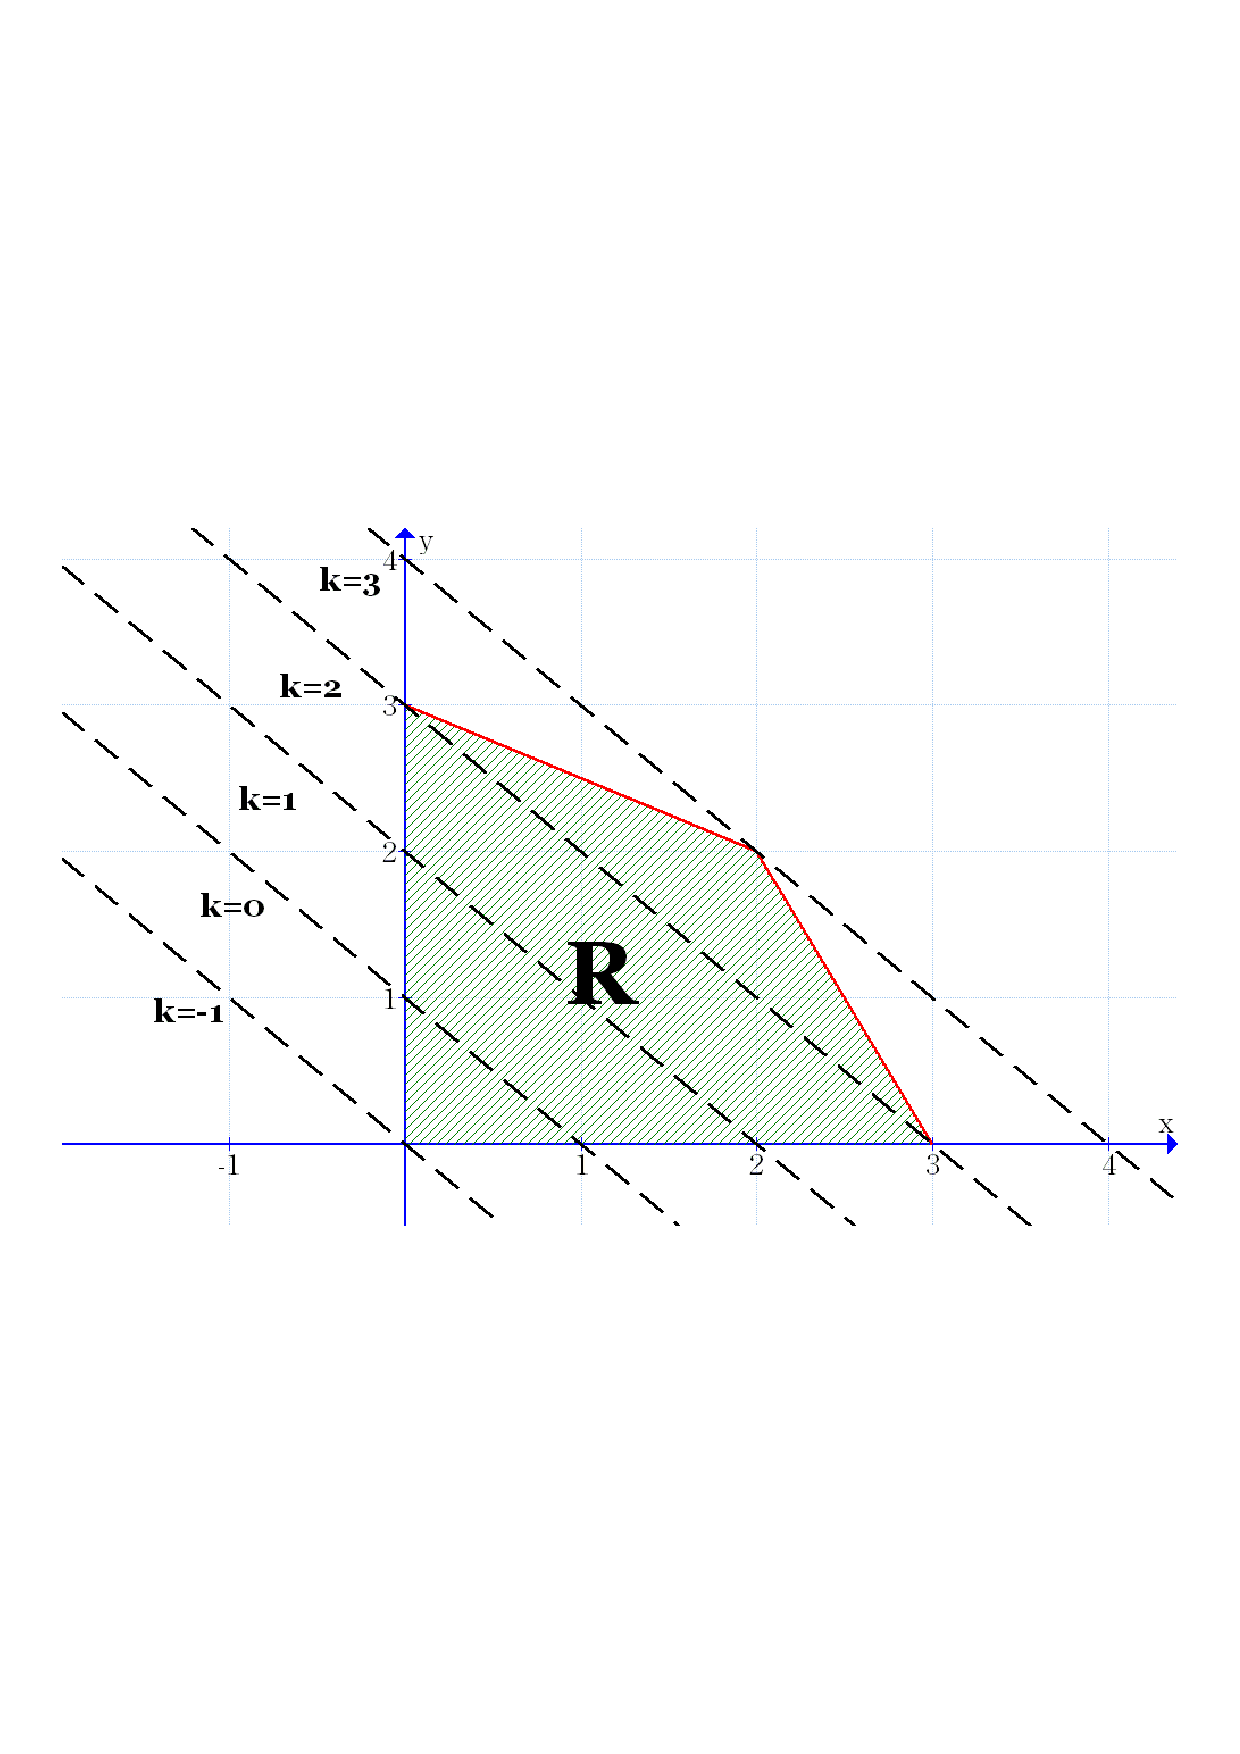
\includegraphics[scale=0.4]{max.pdf}}} \fi

\item At which point will $f(x,y)$ achieve an absolute maximum value?  And, what is this maximum value?

\ifans{\fbox{$f$ achieves its maximum at $(2,2)$.  The maximum value is $3$.}} \fi

\item At which point will $f(x,y)$ achieve an absolute minimum value?  And, what is this minimum value?

\ifans{\fbox{$f$ achieves its minimum at $(0,0)$.  The maximum value is $-1$.}} \fi

\end{enumerate}

\end{enumerate}

\end{document}